\chapter{Vacuum polarization}

\section{The setup}
\note{This first order backreaction calculation should only be valid up to $\varepsilon \lambda \ll 1$ (?). In the problem of a charged particle of charge $e$ colliding with a nucleus of charge $Ze$, vacuum polarization becomes relevant when the coupling constant becomes comparable to the source. Where to discuss this? What when this approximation isn't true?}

We study the coupling of a massive charged scalar complex field $\phi$ to a classical external electromagnetic field $A_\mu$ in a 1+1 dimensional flat spacetime. The simplest description this admits is the minimal coupling of the scalar field to the background classical gauge field $A_\mu$
\begin{align}
	S [\phi, A_\mu] = \int_{\mathbb{R}^2}^{} dx^{0}dx^{1} \left( \frac{1}{2}D_\mu \phi D^*^{\mu}\phi^* 
	+ \mu^2\phi^* \phi - \frac{1}{4}F_{\mu\nu} F^{\mu\nu} + A_\mu j_{\text{external}}^{\mu} \right)  	
	\label{eq:KGM-action}
\end{align}
\note{This shows $\mathcal{L}$. Relevant to write the corresponding Hamiltonian density?} \\
with $D_\mu = \partial_\mu + ieA_\mu$ the gauge covariant derivative given by the minimal coupling to $A_\mu$ and  $e$, $\mu$ the charge and mass parameter of the Klein-Gordon field, respectively. $F_{\mu\nu} = \partial_\mu A_\nu - \partial_\nu A_\mu$ is the electromagnetic stress-energy tensor and $j_{\text{external}}^\mu$ is the charge current density of the external source.

From \eqref{eq:KGM-action}  one derives through the Euler-Lagrange equations the Klein-Gordon-Maxwell equations, namely the coupled system of differential equations given by the Klein-Gordon equation and the Maxwell equations
\begin{subequations}
	\begin{align}
			\left( D_\mu D^\mu + \mu^2  \right) \phi = 0 
		\label{eq:klein-gordon-equation}\\
			\partial_\mu F^{\mu\nu}= j_{\text{external}}^{\nu} + j_\text{br}^{\nu} ,
		\label{eq:quantum-maxwell-equation}
	\end{align}
\end{subequations}
with 
\begin{align}
	j^{\nu}_{\text{br}} = ie\left( \phi^* D_0 \phi - \phi D_0^* \phi^* \right) 
\end{align}
the charge current density of the Klein-Gordon field. 


This set up attempts to act as a toy model for studying Quantum Field Theory on Curved Spacetimes (QFTCS), which is concerned in the study of quantum fields on fixed background spacetimes. For these fields one can calculate its stress-energy tensor $T_{\mu\nu}$, which acts as a gravitational source.  $T_{\mu\nu}$ is not necessary 0 and will therefore have a non-zero contribution to the gravitational field. The semi-classical ansatz is assuming that the contribution of the quantum field to the Einstein field equations is through its expectation value
\begin{align}
R_{\mu\nu} + \frac{1}{2}Rg_{\mu\nu} = 8\pi \left( T_{\mu\nu} + \left<T_{\mu\nu}^\text{br} \right>_\omega \right),
\end{align}
in which the field acts as a source for the gravitational field through its expectation value in a state $\omega$. The 'quantum' contributions to the metric are assumed to be irrelevant when the spacetime curvature is less than the Planck scale.

In a similar fashion, we study the semi-classical Maxwell equations 
\begin{align}
			\partial_\mu F^{\mu\nu}= j_{\text{external}}^{\nu} + \left<j_\text{br}^{\nu} \right>,
			\label{eq:semi-classical-maxwell}
\end{align}
to see how the back-reaction of the Klein-Gordon field affects the background electromagnetic field. 

The background electric field in the region we are studying $[0, a]$ is generated by two charges $q, -q$ placed at the boundaries. Placing the positive charge at the left boundary and the negative charge at the right boundary generates a constant, time-independent electric field $E=q$ pointing towards positive $x^{1}$.
Equation \eqref{eq:klein-gordon-equation} can be solved with attractive or repulsive boundary conditions, resp. Dirichlet $\left. \phi\right|_{x^1 = 0, a}=0$, Neumann $\left. \partial_{1}\phi\right|_{x^1 = 0, a}=0$ , or Robin boundary conditions $\left.\left( \partial_1 + h\right)\phi  \right|_{x^{1}=0, a}=0$ with the $h\in \mathbb{R}$ appropiately chosen at each boundary. Equation \eqref{eq:semi-classical-maxwell} need however be solved with Dirichlet boundary conditions.

\subsection{Gauge fixing}

The charge current density in the laboratory frame of reference is $j^{\nu}=(\rho, 0)$.
%The Maxwell equations read 
%\begin{align}
%	\begin{split}
%		\partial_\mu \partial^\mu A^{0}- \partial_\mu \partial^0 A^{\mu} &= \rho \\
%		\partial_\mu \partial^\mu A^{1}- \partial_\mu \partial^1 A^{\mu} &= 0
%	\end{split}
%\end{align}
We therefore choose to  solve this problem using Coulomb gauge, $\partial_1 A_1 = 0$. In this gauge, the space component $A_1$ of the vector potential is 0 up to an addition constant, and 
we turn our attentions to the time component $A_0$ of the vector potential. In the Coulomb gauge, for $x^{1}\in (0, a)$, $A_0$ solves the Poisson equation
\begin{align}
	 \partial_1^2 A_0 = -\rho 
	 \label{eq:poisson}
\end{align}
Equation \eqref{eq:poisson}  is to be solved with the boundary conditions
\begin{align}
 	  \left.\partial_1 A_0 \right|_{x_1=0, a}=-E,
		  \label{eq:boundary-conditions-A0}
\end{align}
so that no screening appears in the boundaries. This fixes the solution up to a constant factor, which is to be chosen so that the problem is antisymmetric. It suffices to demand $A_0(\frac{a}{2}) = 0$.

For clarity, we artificially split the full potential $A_0$ into two: $A_0^\text{external}$ due to the constant background electric field and $A_0^{\text{br}}$ due to the backreaction of the Klein-Gordon field.
Hence, \eqref{eq:poisson} splits into  
\begin{align}
	\begin{split}
		\partial_1^2A_0^{\text{external}}&= 0 \\
		\left.\partial_1 A_0^{\text{external}} \right|_{x_1=0, a}&=-E,
	\end{split}
			\label{eq:poisson-external}
		\end{align}
	and
\begin{align}
	\begin{split}
		\partial_1^2A_0^{\text{br}}&= -\rho \\
		\left.\partial_1 A_0^{\text{br}} \right|_{x_1=0, a}&=0.
	\end{split}
			\label{eq:poisson-br}
		\end{align}
This splitting of the potential makes it clear to write the solution to equation \eqref{eq:poisson} is the full potential
		\begin{align}
			A_0(x^{1}) &=
			A_0^{\text{external}}(x^{1}) +
			A_0^{\text{br}}(x^{1}) =  \\
				   &-E\left( x^{1}-\frac{a}{2} \right) - \int_{\frac{a}{2}}^{x^{1}}\int_{0}^{x^{1}'}     \rho(x^{1}'') dx^{1}'' dx^{1}' .
		\end{align}


		Knowing how to calculate $A_0$ (provided we know how to calculate $\rho_\phi$) we can now write \eqref{eq:klein-gordon-equation} as 
		\begin{align}
			\left( -(\partial_0 +ie A_0(x^{1}))^2 + \partial_1^2 + m^2 \right) \phi = 0.
			\label{eq:TDKGE}
		\end{align}

Finally, define the dimensionless parameters 
		\begin{align}
			\begin{split}
				(t, z) := \left(\frac{x^{0}}{a}	,\frac{x^{1}}{a}	  \right) \\
				\begin{tabular}{cc}
					\lambda = ea^2E  &
				\varepsilon = ae \\
				m = a\mu & 
				\omega_n = a\Omega_{n, \alpha} + \lambda \alpha,
				\end{tabular}
%				\lambda &= ea^2E \\
%				\varepsilon &= ae \\
%				m &= a\mu \\
%				\omega_n &= a\Omega_n,
			\end{split}
		\end{align}
		and use the ansatz
		$	\phi(t, z) = \phi_n(z) e^{-i\omega_n t},$
		to split \eqref{eq:TDKGE} into the dimensionless mode equations 
		\begin{align}
			\left( (\omega_n - \varepsilon A_0 )^2 + \frac{d^2}{dz^2}- m^2 \right) \phi_n = 0.
		\label{eq:TIKGE}
		\end{align}
		Each of the modes is normalised with respect to the inner product
		\begin{align}
			(\phi_n, \phi_m) = i \int_{0}^{1} dz \left( \pi^*_n \phi^*_m - \pi_m \phi_n \right),
			\label{eq:symplectic-inner-product}
		\end{align}
		with $\pi_n^* = D_0\phi_n$ the canonical conjugate of $\phi.$ Positive (negative) energy solutions are normalized to $+1$ ($-1$).

\section{The external field approximation}
To study the relevance of the backreaction of the scalar field we first study the external field approximation, ignoring the backreaction of the scalar field. In this approximation, $A_0(z) = -\lambda \left( z-\frac{1}{2} \right) $, and therefore equation \eqref{eq:TIKGE} takes the form
		\begin{align}
			\left( \left[(\omega_n + \lambda\left( z-\frac{1}{2} \right)\right] ^2 + \frac{d^2}{dz^2} - m^2 \right) \phi_n = 0.
			\label{eq:klein-gordon-in-the-external-field-approximation}
		\end{align}

		With the appropriate parameter definitions, 
		\begin{align}
			x = \frac{1+i}{\sqrt{\lambda} } \left[ \omega_n + \lambda \left(z - \frac{1}{2}\right) \right] , \,\,\,\,\,\, n = -\frac{m^2}{2\lambda} - 1/2,
		\end{align}
		equation \eqref{eq:klein-gordon-in-the-external-field-approximation}  can be identified with the Weber equation 
		\begin{align}
			 \frac{d^2 D_n(x)}{dx^2} + \left(n+ \frac{1}{2 }-\frac{1}{4}x^2\right) D_n(x) = 0,
			 \label{eq:Weber-equation}
		\end{align}
		which is solved by the parabolyc cylinder functions $D_n(x)$ [citation required].
		Equation \eqref{eq:klein-gordon-equation} is then solved by 
\begin{align}
	\begin{split}
	\phi_n(z) &= 
	a_n D_{i \frac{m_a^2}{2\lambda} - \frac{1}{2}} \left( 
		\frac{1+i}{\sqrt{\lambda} }
		\left( \omega_n + \lambda \left( z-\frac{1}{2} \right)
		\right) 
	\right)  \\
	&+
	b_n D_{-i \frac{m_a^2}{2\lambda} - \frac{1}{2}} \left( 
		\frac{i - 1}{\sqrt{\lambda} }
		\left( \omega_n + \lambda \left( z-\frac{1}{2} \right)
		\right) 
	\right),
	\end{split}
	\label{eq:parabolyc-cylinder}
\end{align}
where the parameters $\omega_n, a_n, b_n$ are to be calculated by applying the corresponding boundary and normalization conditions for the field $\phi_n$.


This approximation presents an instability in the sense that when increasing the external electric field strength $\lambda$ past a certain critical value $\lambda_c$, the vacuum polarization diverges and the energy of the modes goes into the complex realm. This leads to runaway solutions, as the complex exponential in the single frequency ansatz $\phi_n(z)e^{i \omega_n t }$ turns into a real exponential \cite{Ambjorn1983}. This instability is shown in figure \ref{fig:figures-eigenvalues-external-field-approximation-png}, where the energy of the first mode is represented, as $\lambda$ goes to $\lambda_c$. \note{Add more modes to the plot?}

\begin{figure}[t]
	\centering
	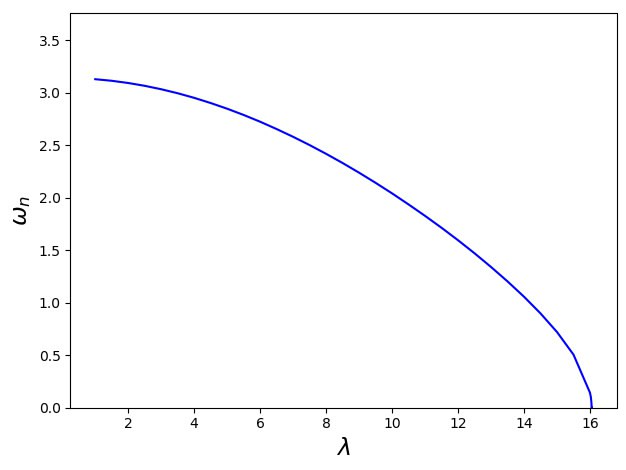
\includegraphics[width=0.8\textwidth]{figures/eigenvalues-external-field-approximation.png}
	\caption{The energy of the first mode as the background electric field strength $\lambda$ is increased, showing the vertical drop to 0 when $\lambda\to \lambda_c$, displaying the is the appearance of the instability. \note{Show the diverging vacuum polarization as $\lambda\to \lambda_c$ }}
	\label{fig:figures-eigenvalues-external-field-approximation-png}
\end{figure}

\cite{Ambjorn1983} claims that the screening nature of the Klein-Gordon vacuum is enough to raise the energy of the modes enough in order to avoid these instabilities. However, the vacuum polarization in \cite{Ambjorn1983} is not calculated properly \cite{Wernersson2020} and therefore the question still stands. As we will see below, in the correct renormalization procedure, the Klein-Gordon vacuum is still screening enough, and the instabilities are therefore avoided.

		\section{Quantization and vacuum polarization}


		We write the solution to equation \eqref{eq:TDKGE} after changing the variables
		\begin{align}
			\phi(t, z) = \sum_{n>0}^{} a_n \phi_n(z) e^{-i\omega_n t} + \sum_{n<0}^{} b_n^\dagger \phi_n^*(z) e^{-i\omega_n t},
			\label{eq:field-expansion}
		\end{align}
		with $a_n$, $b_n$ the annihilation operators for the positive and negative energy solutions, respectively. These operators obey the commutation relations 
		\begin{align}
			[a_n, a_m^\dagger] =
			[b_n, b_m^\dagger] = \delta_{nm},
		\end{align}
		with all other possible commutators vanishing. These operators define the vacuum state $\ket{0} $ 
		\begin{align}
			a_n \ket{0} = b_n \ket{0} = 0.
		\end{align}

		The vacuum polarization is calculated as
		\begin{align}
			\rho(z) = i\varepsilon \vacuum{ \phi^* D_0\phi - \phi D_0^* \phi^* }.
			\label{eq:vacuum-polarization}
		\end{align}
		$\phi$ is an operator valued distribution.
		Evaluating products of distributions at the same points is a priori ill-defined, and the expectation value in \eqref{eq:vacuum-polarization}  should be calculated as explained in section \ref{sec:Hadamard}, i.e. by defining the expectation value of products of (derivatives of) fields at the same point via point-splitting with respect to the Hadamard parametrix as in \eqref{eq:point-splitting-wrt-a-Hadamard-parametrix}.
		The Hadamard parametrix $H(x, x') $ of the Klein-Gordon field in 1+1 dimensions up to relevant order\footnote{The charge density operator only has first order derivatives, and therefore higher orders in the Hadamard parametrix will vanish after taking the limit $x'\to x$ } is given by
		\begin{align}
			H^{\phi^* \phi}(x, x') = -\frac{1}{4\pi}U(x, x') \ln \sigma_\varepsilon,
		\end{align}
	with $\sigma = \frac{1}{2}(x - x')^2$ the geodesic distance between $x$ and $x'$, and $\sigma_\varepsilon = \sigma + i \varepsilon (t-t')$, where the limit $\varepsilon\to 0^+$ is to be taken at the end of the calculation.

	The smooth coefficient $U(x, x')$  is calculated by parallely transporting it with respect to $D_\mu$ along the geodesic (straight line) joining $x$ and $x'$. This results in 
	\begin{align}
		U(x, x') = \exp \left( -i\varepsilon \int_{0}^{1} A_\mu(x' + s(x-x')) \left( x- x' \right) ^{ \mu} ds  \right) .
	\end{align}
	In the chosen gauge $A_\mu(t, z) = (A_0(z), 0)$, and performing the point-splitting in the time direction, $x' =  (t+\tau, z)$, 
	\begin{align}
	U(x, x') = \exp\left( -ie\tau A_0(z) \right).
	\end{align}

We calculate the vacuum expectation value of the first term in equation \eqref{eq:vacuum-polarization}.  In this point-splitting, the two-point function  $w_0^{\phi^*\phi }(x, x')$ takes the form
	\begin{align}
		w^{\phi^* \phi}(x, x') = \vacuum{\phi^*(x) \phi(x')} = \sum_{n<0}^{} \abs{\phi_n(z)}^2 e^{-i \omega_n \left( \tau + i\epsilon \right) },
	\end{align}
where an $i \epsilon$-prescription is used in order to ensure convergence. The derivative of $w^{\phi^* \phi}(x, x')$ with respect to the time coordinate of $x'$ reads
\begin{align}
	D_0'w^{\phi^* \phi}(x, x') &= -i \sum_{n<0} (\omega_n - eA_0(z))\lvert \phi_n \rvert ^2 e^{-i\omega_n (\tau+i\epsilon)},
\end{align}
and of the parametrix $H^{\phi^* \phi}$,
\begin{align}
	D_0' H^{\phi^*\phi}(x, x') &= -\frac{1}{2\pi}\frac{1}{\tau + i\varepsilon} - \frac{ieA_0(z) }{2\pi} + \mathcal{O}(\tau).
\end{align}
This implies 
\begin{align}
\vacuum{  \phi(x)^* D_0\phi(x)}  = \lim_{\tau \to 0} 
 -i\sum_{n<0}^{} (\omega_n - eA_0)\abs{\phi_n(z)}^2 e^{-i \omega_n \left( \tau + i\epsilon \right) }
+\frac{1}{2\pi}\frac{1}{\tau + i\varepsilon} - \frac{ieA_0(z) }{2\pi} + \mathcal{O}(\tau).
\end{align}

Similarly, for the second term in \eqref{eq:vacuum-polarization}, 
\begin{align}
	D_0^*'w^{\phi\phi^* }(x, x') &= i \sum_{n>0} (\omega_n - eA_0(z))\lvert \phi_n \rvert ^2 e^{i\omega_n (\tau+i\epsilon)},
\end{align}
and
\begin{align}
	D_0^*' H^{\phi\phi^*}(x, x') &= -\frac{1}{2\pi}\frac{1}{\tau + i\varepsilon} + \frac{ieA_0(z) }{2\pi} + \mathcal{O}(\tau),
\end{align}
since $U^*(x, x') = U(x', x)$.
This implies 
\begin{align}
\vacuum{  \phi(x)D_0\phi(x)^* }  = \lim_{\tau \to 0} 
 i\sum_{n>0}^{} (\omega_n - eA_0)\abs{\phi_n(z)}^2 e^{i \omega_n \left( \tau + i\epsilon \right) }
+\frac{1}{2\pi}\frac{1}{\tau + i\varepsilon} - \frac{ieA_0(z) }{2\pi} + \mathcal{O}(\tau).
\end{align}

When subtracting these two quantities as per \eqref{eq:vacuum-polarization}, the divergent terms cancel each other out, resulting in the following expression for the vacuum polarization 
\begin{align}
	\begin{split}
			&\rho(z) =  \\
			&\lim_{\tau \to 0}\left(
			\sum_{n< 0}^{} (\omega_n - A_0) \|\phi_n\|^2 e^{-i \omega_n (\tau + i\varepsilon)}  +
			\sum_{n> 0}^{} (\omega_n - A_0) \|\phi_n\|^2 e^{i \omega_n (\tau + i\varepsilon)}  \right)
			+ \frac{e^2}{\pi} A_0(z).
	\end{split}
	\label{eq:Hadamard-vacuum-polarization}
\end{align}
This expression is gauge independent, as long as the summation and the limit  are taken in the correct order. 

In \cite{Ambjorn1983}, the vacuum polarization is calculated as 
\begin{align}
	\begin{split}
			\rho(z) =  
			\sum_{n< 0}^{} (\omega_n - A_0) \|\phi_n\|^2 + 
			\sum_{n> 0}^{} (\omega_n - A_0) \|\phi_n\|^2 ,
	\end{split}
\end{align}
which even though it is gauge invariant, it cannot be derived from a gauge invariant theory. The crucial difference is the extra $\frac{\varepsilon^2}{\pi} A_0(z)$.

\subsection{Perturbation theory}
\note{Q: I find that this calculations are necessary for some reasons:
	\begin{enumerate}
		\item To have an intuition on how the vacuum polarizes on this setup
		\item To show the difference between the mode sum and the Hadamard point-split formula 
		\item Knowing this difference, that the answer to the question "does backreaction avoid instabilities?" is not obvious.
	\end{enumerate}
However, I am basically copying the results from the bibliography, and I do not want to do that. Should I keep this section? Or just cite it?
}
%Following the steps of \cite{Ambjorn1983, Wernersson2020}
%, it might be instructive to study the problem perturbatively. We state the problem as a Schrödinger-like equation 
%\begin{align}
%	i \partial_t \ket{\Psi} = H \ket{\Psi}
%	\label{eq:schrodinger}
%\end{align}
%with 
%\begin{align}
%	\ket{\Psi} = \begin{pmatrix} \phi \\ \pi^* \end{pmatrix}, 
%\text{and }\pi^* = D_0 \phi.
%\end{align}
%The space of all $\ket{\Psi}$ equipped with the inner product  \eqref{eq:symplectic-inner-product} forms the phase space of our system.
%
%We can construct the corresponding Hamiltonian operator as 
%\begin{align}
%	H= i \begin{pmatrix} 
%	0 & 1 \\
%	D_1 ^2 - m^2 & 0
%\end{pmatrix}
%+ \begin{pmatrix}  
%	eA_0 & 0 \\
%	0 & eA_0
%\end{pmatrix} 
% = H_0 + H_1.
%\end{align}
%The Hamiltonian $H$ is split into a free field hamiltonian $H_0$ and consider $H_1$ to be a perturbation. $H$ is hermitean with respect to the inner product \eqref{eq:symplectic-inner-product}.
%The eigenstates $\Psi_n$ of $H_0$ with eigenvalues $\omega_n$ are the solutions to a free particle in a box  f size 1. For Dirichlet boundary conditions ($\Psi(0) = \Psi(1) = 0$),
%\begin{align}
%	\omega_n^D = \text{sign}(n) \sqrt{m^2 + \pi^2 n^2} ,\hspace{1cm} \phi_n^D(z) = \lvert \omega_n \rvert ^{-\frac{1}{2}} \sin \pi n z,
%	\hspace{0.3cm}	n \in \mathbb{Z} \setminus \{0\} ,
%\end{align}
%For Neumann boundary conditions $(\Psi'(0) = \Psi'(1) = 0)$ one has 
%\begin{align}
%	\omega_{n \neq 0}^N = \text{sign}(n) \sqrt{m^2 + \pi^2 n ^2},
%	\hspace{0.4cm}	& \phi^N_{n\neq 0} (z) = \lvert \omega_n \rvert ^{- \frac{1}{2}}\cos \pi n z \\
%	\omega_{\pm 0}^N = \pm m,
%	\hspace{0.4cm}	& \phi^N_{\pm 0} (z) = \left( 2m \right) ^{-\frac{1}{2}}.
%\end{align}
%These eigenstates are the zeroth order correction $\ket{\Psi_n^{(0)}}$ to the $H_0$ eigenstates. The first order correction is given by perturbation theory  
%\begin{align}
%	\omega_n ^{(1)} &= \frac{\bra{\Psi_n^{(1)}}\ket{H_1\Psi_n^{(1)}}}{\bra{\Psi_n^{(0)}}\ket{\Psi_n^{(0)}}} \\
%	\ket{\Psi_n ^{(1)}} &= \sum_{k\neq n}^{} 
%	\frac{
%		1
%	}
%	{
%	\bra{\Psi_n^{(0)}}\ket{\Psi_n^{(0)}}
%	}
%	\frac{
%	\bra{\Psi_k^{(0)}}\ket{H_1\Psi_n^{(0)}}
%	}{
%	\omega_n ^{0} - \omega_k^{(0)}
%	} \ket{\Psi_k^{(0)}}
%\end{align}

It might be enlightening to see the mode solutions and vacuum polarization at first perturbational order. These calculations were already done in \cite{Ambjorn1983, Wernersson2020}, and we therefore just state the perturbative corrections to the free field solutions, for Dirichlet boundary conditions (marked with a superscript D) and for Neumann boundary conditions (marked with a superscript N). 
\begin{align}
	\begin{split}
	\phi_n^{D} &= \left( m^2 + \pi^2  n^2 \right)^{-\frac{1}{2}} \Biggl[ \sin\pi n z \\
		   &\left.+ \lambda \frac{\sqrt{m^2 + \pi^2 n^2} }{2 \pi \lvert n \rvert} 
		\left( 
		\frac{1}{\pi n}\left( \frac{1}{2} - z \right) \sin \pi n z - z(1-z) \cos \pi n z \right) 
	\right] 
	\end{split} 
	\label{eq:perturbative-dirichlet}
	\\
	\begin{split}
	\phi_n^{N} &= \left( m^2 + \pi^2 n^2 \right)^{-\frac{1}{2}} 
	\Biggl[ \cos\pi n z  \right. \\
		   &\left. + \lambda \frac{\sqrt{m^2 + \pi^2 n^2} }{2 \pi \lvert n \rvert} 
		\left( 
		\frac{1}{\pi n}\left( \frac{1}{2} - z \right) \cos \pi n z 
	+ ( z(1-z) + (\pi n)^{-2)} ) \sin \pi n z \right) 
	\right] 
	\end{split}
	\label{eq:perturbative-neumann}
	\\
	\begin{split}
	\phi_{\pm 0 }^{N} &= \left( 2m \right) ^{- \frac{1}{2}} \mp \lambda \sqrt{2m} \left( \frac{1}{24} - \frac{1}{4}z^2 + \frac{1}{6}z^3\right).
	\end{split}
	\label{eq:perturbative-neumann-n-0}
\end{align}

\subsection{Vacuum polarization at first order in perturbation theory}
Using \eqref{eq:Hadamard-vacuum-polarization} we calculate the vacuum polarization at first order in $\lambda$ for the massless case using Dirichlet boundary conditions. We rewrite \eqref{eq:Hadamard-vacuum-polarization} as 
\begin{align}
\rho(z) = \vareprilon \lim_{\tau\to 0} \sum_{n=1}^{\infty} \left( \lvert \phi_n\rvert ^2 (\pi n - \varepsilon A_0) - \lvert \phi_{-n}\rvert ^2 (\pi n + \varepsilon A_0) \right)  e^{i \pi n (\tau + i \epsilon)} + \frac{e^2}{\pi}A_0.
\label{eq:perturbative-vacuum-polarization}
\end{align}

From \eqref{eq:perturbative-dirichlet}, up to first order in $\lambda$,
\begin{align}
	\lvert \phi_n\rvert ^2 = \frac{1}{\pi\|n\|} \left( \sin^2\pi n z - \lambda \sin\pi n z \left[ \frac{1}{\pi n } \left( z - \frac{1}{2} \right) \sin \pi n z + z (1- z) cos \pi n z\right]  \right) .
\end{align}
Substituting in \eqref{eq:perturbative-vacuum-polarization}, and with some rearranging, 
\begin{align}
	\begin{split}
		\rho(z) &= -2\varepsilon \lambda \lim_{\tau \to 0} \sum_{n=1}^{\infty} z(1-z) \sin \pi n z  \cos \pi nz - \frac{\lambda}{\pi} \left( z-\frac{1}{2} \right) \\
		&= -\varepsilon \lambda  z(1-z) \lim_{\tau \to 0} \frac{1}{2i} 
		\left(
			\frac{e^{i \pi (2 z + \tau + i\epsilon)}}{1 - e^{i\pi( 2z + \tau + i\epsilon) }} 
			- \frac{e^{i \pi (-2 z + \tau + i\epsilon)}}{1 - e^{i\pi( -2z + \tau + i\epsilon) }} 
		\right) 
		- \frac{\lambda}{\pi} \left( z-\frac{1}{2} \right) \\
		&= -\varepsilon \lambda  z(1-z) \cot \pi z	- \frac{\lambda}{\pi} \left( z-\frac{1}{2} \right).
	\end{split}
\end{align}
In \cite{Ambjorn1983}, the vacuum polarization at first order in $\lambda$ is (wrongly) calculated as 
\begin{align}
	\rho  =  - 2 \varepsilon\lambda z (1-z) \cot(\pi z).
\end{align}

\begin{figure}[t]
	\centering
	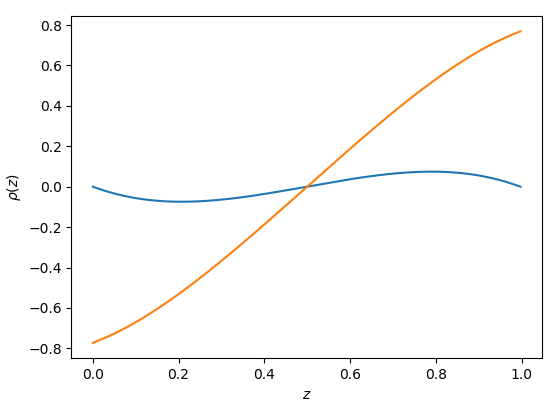
\includegraphics[width=0.8\textwidth]{figures/renormalization_comparison_rho.png}
	\caption{The vacuum polarization at first order in $\lambda$ in Dirichlet boundary conditions. In orange, $\rho$ as calculated using the mode sum in \cite{Ambjorn1983}, and in blue using point splitting with respect to the Hadamard parametrix as in \cite{Wernersson2020}. \note{Here I intend to add a third curve, with the mode sum formula for $\rho$ for $N=1$, which is the one used in \cite{Ambjorn1983}.}}
	\label{fig:perturbative-rho-comparison}
\end{figure}
We show in the figure \ref{fig:perturbative-rho-comparison} the comparison between the two $\rho$. Notice how the addition of the potential term in \eqref{eq:Hadamard-vacuum-polarization} forces $\rho$ to be 0 at the boundaries, as one would expect for Dirichlet boundary conditions. We also observe that the overall vacuum polarization is much stronger when calculating it using the mode sum formula. The main claim in  \cite{Ambjorn1983}, is that when considerring the back reaction of the scalar field, the instabilities that appear in the external field approximation disappear. However, since \cite{Ambjorn1983} uses a wrong expression to calculate the back-reaction of the scalar field, and the correct expression leads to a much 'weaker'  $\rho$, it is not obvious to say whether the back-reaction of the field is enough to raise the energy of the modes enough so as to avoid the original instabilities.
\section{The iterative procedure}

To include backreaction into the calculation, we proceed iteratively.
Following the convention used in \cite{Ambjorn1983}, we label by $\kappa$ each of the iterations. For a given $A_0^{\kappa}$, at each step $\kappa$ we solve numerically the following equations,
\begin{align}
	\partial_1^2 \phi^{\kappa+1}_n &=
	\left( - (\omega^{\kappa+1}_n - \varepsilon A^{\kappa}_0(z))^2 + m^2 \right) \phi^{\kappa+1}_n
	\label{eq:iterative-TIKGE}\\
	\begin{split}
		\varepsilon A_0^{\kappa}(z) &= -\lambda\left( z-\frac{1}{2} \right)  - \varepsilon\int_{\frac{1}{2}}^{z} \int_{0}^{z'} \rho^{\kappa}(z'')  dz'' dz'\\
		\varepsilon A_0^{0}(z) &= -\lambda\left( z-\frac{1}{2}\right) 
	\end{split}
	\label{eq:potential-at-step-kappa}
.
\end{align}
with $\rho$ calculated using \eqref{eq:Hadamard-vacuum-polarization}, up to a finite mode cutoff in the sum. This cutoff at mode N causes the calculated $\rho$ to be oscillatory, of period $\Delta z = \frac{1}{N+1}$, which should be averaged out.

Finally, we take the limit $\kappa \to \infty$, i.e. solve equation \eqref{eq:iterative-TIKGE} for a given potential $A_0^{\kappa}$, calculate the corresponding induced potential at $\kappa$, and solve equation \eqref{eq:iterative-TIKGE} using this new potential. We look for convergence following this procedure. The computation is halted when convergence with respect to some norm is found. Once a self-consistent solution is found, we use this solution as a guess for some new $\lambda$ value, greater than the old one. In this way, we sample the whole $\lambda$-parameter space to study the interaction between the scalar field and the external electric field. 

This procedure can be also be stated in terms of infinite dimensional fixed point problems,
\begin{align}
	A_0 = f(A_0),
\end{align}
with $f$ the update rule given by equation \eqref{eq:potential-at-step-kappa}. The function $f$ has no closed form, as calculating $\rho$ in \eqref{eq:potential-at-step-kappa} involves taking all the steps that were explained throughout this section. 

\subsection{Numerical instabilities}
Even though we are considering the back-reaction of the field, this problem still presents some instabilities when crossing $\lambda\approx \lambda_c$. When sampling the $\lambda$-parameter space, if the step  $\Delta \lambda$ is too big, then one of two things might happen:
\begin{enumerate}
	\item Since we are using the previous solutions as the initial guess to find the self-consistent solution, the screening from the previous solution might not be strong enough causing the energies of some modes to not have solutions in $\mathbb{R}$, or
	\item convergence is too slow.
\end{enumerate}
Even though this can in theory be overcome by choosing smaller $\Delta \lambda$, in practice $\Delta \lambda$ can get to the order of  $10^{-7}$. At $\sim 30s $ per value of $\lambda$, this amounts to about 10 years to  achieve a step of unit size in $\lambda$.

To overcome this, we slightly modify the iterative procedure with a \textit{relaxing} procedure, 
\begin{align}
	A_0^{\kappa+1}(z) = c A_0^{\kappa}(z)+ (1-c) \left[ -\lambda \left( z-\frac{1}{2} \right) - \int_{\frac{1}{2}}^{z} \int_{0}^{z'} \rho^{\kappa} (z'') dz'' dz'   \right], \,\,\, 0< c \lesssim 1.
\end{align}
This scheme avoids these instabilities by allowing self consistent solutions to "relax" into one another, i.e. if for a certain $\lambda$ value a self-consistent solution is found but $\Delta \lambda$ was too big, the change in the potential will not be as strong as it was in the previous scheme. The closer the parameter $c$ is to 1, the slower the convergence, but the more relaxed.

\section{Computational details}

\subsection{Noise filtering}
To solve this problem numerically, we split the interval $(0, 1)$ into M equal intervals, with the mesh points $0<\ldots<z_i<\ldots<1$ and  $i\in \left[ 0, M-1 \right] $.

In the (numerical) computation of \eqref{eq:Hadamard-vacuum-polarization} one needs to cut the mode sum at some finite mode N. This induces oscillations of period $\Delta z = \frac{1}{N + 1}$ in the resulting vacuum polarization, which should be averaged out. To do this, we convolute the resulting $\rho$ with a very specific array, designed to cancel these oscillations out. 
Recall the definition of the convolution of two arrays $\rho_n$, $b_n$ not necessarily of the same length
\begin{align}
	(\rho*b)_n = \sum_{n=0}^{M} \rho_m b_{n-m}.
\end{align}
A convoluting array of the form\footnote{It should be renormalized so that the sum of its elements is 1}
\begin{align}
	b_n = \left[ 1, 0 , 4 , 0 , 6 , 0,4,0,1 \right] 
\end{align}
approximately cancels the oscillations. For this to be effective, this array should "fit" exactly one period of the noise oscillations, and therefore the number of mesh points should be exactly $M = 8 (N + 1)$.
